%%%%%%%%%%%%%%%%%%%%%%%%%%%%%%%%%%%%%%%%%%%%%%%%%%%%%%%%%%%%%%
\section{Geometry-based Analysis}\label{sec:2}
%%%%%%%%%%%%%%%%%%%%%%%%%%%%%%%%%%%%%%%%%%%%%%%%%%%%%%%%%%%%%%

\subsection{Key Data}

The structures used to support the problem definition, the discretization of the
model and their interactions are central to mesh-based analysis methods like
finite element and finite volumes.  The geometry-based analysis environment consists of four parts: \emph{the geometric model} which houses the topological and shape description of the domain of the problem,
\emph{attributes} describing the rest of information needed to define and solve the
problem, \emph{the mesh} which describes the discretized representation of the
domain used by the analysis method, and \emph{fields} which describe the
distribution of solution tensors over the mesh entities~\cite{beallthesis, simmetrixweb}.
Figure~\ref{fig:compo} represents the general interactions between the four
components. 

\begin{figure}
\centering
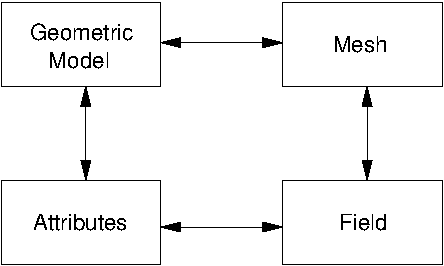
\includegraphics[width=2.5in]{../fig/compo_env}
\caption[The relationship between components of the geometry-based analysis environment]
{The relationship between components of the geometry-based analysis environment~\cite{beallthesis}}
\label{fig:compo}  % the \label command comes AFTER the caption
\end{figure}

%%%%%%%%%%%%%%%%%%%%%%%%%%%%%%%
\subsubsection{Geometric model}
%%%%%%%%%%%%%%%%%%%%%%%%%%%%%%%

\begin{figure}
\centering
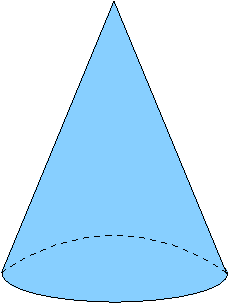
\includegraphics[height=1.3in]{../fig/manifold}\hspace{.5in}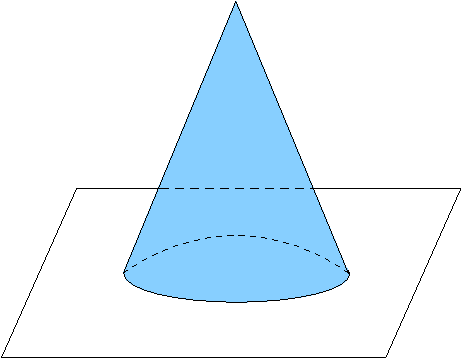
\includegraphics[height=1.5in]{../fig/nonmanifold}
\caption[Example of manifold and non-manifold models]
{Example of (left) manifold and (right) non-manifold models}
\label{fig:nonmanifold}  % the \label command comes AFTER the caption
\end{figure}

The most common geometric representation is a boundary representation. A general
representation of general non-manifold domains is the Radial Edge Data
Structure~\cite{weiler88}. Non-manifold models are common in engineering analyses. Simply speaking,
non-manifold models consist of general combinations of solids, surfaces, and
wires. Figure~\ref{fig:nonmanifold} illustrates examples of manifold and
non-manifold model.

In the boundary representation, the model is a hierarchy of topological entities
called regions, shells, faces, 
loops, edges, vertices, and in case of non-manifold models, use entities for vertices, edges, loops, and
faces.  %The use of a boundary representation is convenient for attribute
%association and mesh generation processes since the 
%boundaries of the model are explicitly represented.
The data structure implementing the geometric model supports operations
to find the various model entities that make up a model, information about which model
entities are adjacent to a given entity, operations relating to perform
geometric shape queries, and queries about what attributes are associated with model
entities.

%%%%%%%%%%%%%%%%%%%%%%%%%%%%%%%
\subsubsection{Attribute}
%%%%%%%%%%%%%%%%%%%%%%%%%%%%%%%

\begin{figure}
\centering
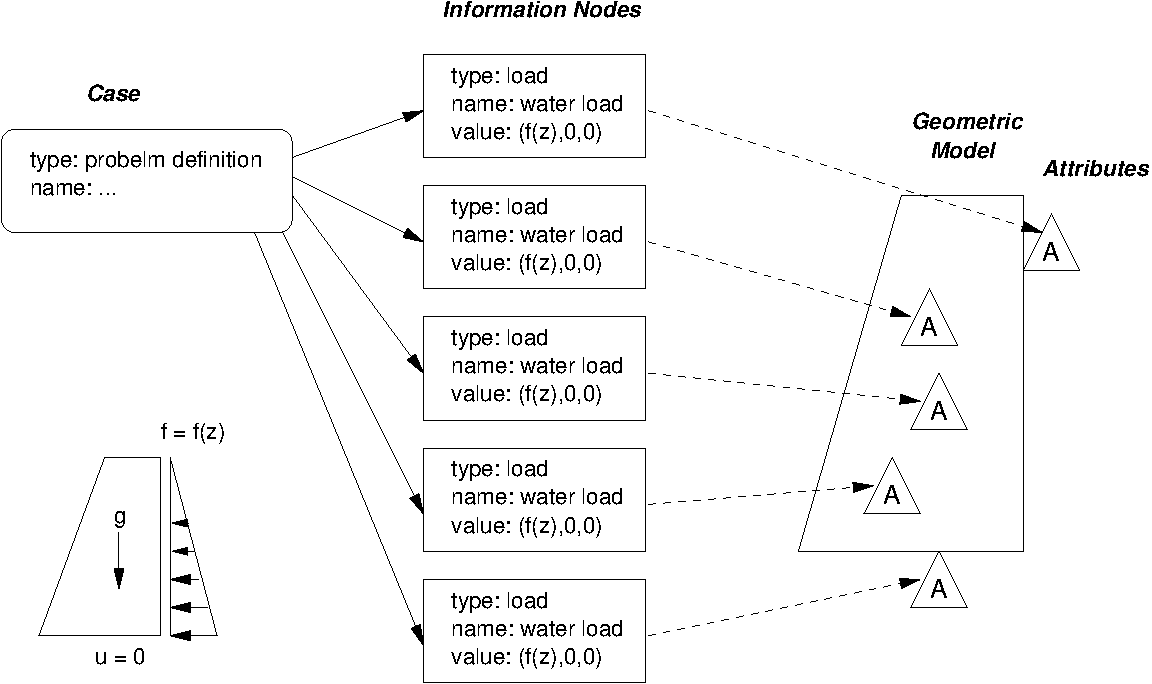
\includegraphics[width=4.5in]{../fig/attributes}
\caption[Example geometry-based problem definition]{Example geometry-based problem definition~\cite{beallthesis}}
\label{fig:dam}  % the \label command comes AFTER the caption
\end{figure}

In addition to geometric model, the definition of a problem requires other information that describes material
properties, loads and boundary conditions, etc. These
are described in terms of tensor-valued 
attributes and may vary in both space and time. Attributes are applied to geometric model entities. 

Figure~\ref{fig:dam} illustrates an example of a problem definition. The problem being modeled is a
dam subjected to loads due to gravity and due to the water behind the dam. There
is a set of attribute information nodes that are all under the attribute case
for the problem definition. When this case is associated with the geometric model,
attributes are created and attached to the individual model entities on which they act~\cite{beallthesis,
simmetrixweb}. The attributes are indicated by triangles with $A$'s inside of them.

%%%%%%%%%%%%%%%%%%%%%%%%%%%%%%%
\subsubsection{Mesh}
%%%%%%%%%%%%%%%%%%%%%%%%%%%%%%%

A mesh is a geometric discretization of a domain. With restrictions on the mesh
entity topology~\cite{beall97}, a mesh is represented with a hierarchy of
regions, faces, edges and vertices. Each mesh entity maintains a relation, called
geometric classification~\cite{beall97, shephard00}, to the model entity that it was
created to partially represent. Geometric classification allows an understanding of which 
attributes (e.g. boundary conditions or material properties) are related to the 
mesh entities and the how the solution relates back to the original problem
description, and is critical in mesh generation and adaptation~\cite{beallthesis, beall97, shephard00}. More discussion on the mesh representation is presented in $\S$2.2. 


In a geometry-based analysis environment, mesh data structures house the
discretization of the domain, a mesh, and provide the mesh-level services to applications. 

%%%%%%%%%%%%%%%%%%%%%%%%%%%%%%%
\subsubsection{Field}
%%%%%%%%%%%%%%%%%%%%%%%%%%%%%%%

\begin{figure}
\centering
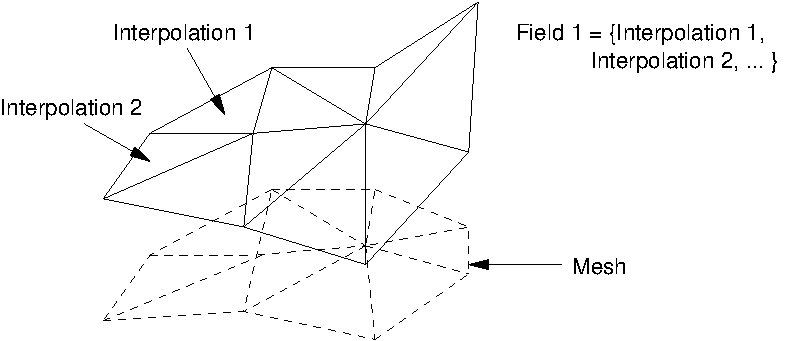
\includegraphics[width=3.5in]{../fig/field}
\caption[Representation of a field defined over a mesh]{Representation of a field defined over a mesh~\cite{beallthesis}}
\label{fig:field}  % the \label command comes AFTER the caption
\end{figure}

A field describes the variation of solution tensors over the mesh entities
discretizing one or more entities in a
geometric model. The spatial variation of the field is defined in terms of
mesh level distribution functions~\cite{beallthesis}.
Figure~\ref{fig:field} demonstrates the concept of a field written in terms of
$C^0$ interpolating distribution functions. 

%%%%%%%%%%%%%%%%%%%%%%%%%%%%%%%%%%%%%%%%%%%%%%%%%%%%%%%%%%%%%%
\subsection{General Topology-Based Mesh Data Structure}\label{ch:genmdb}
%%%%%%%%%%%%%%%%%%%%%%%%%%%%%%%%%%%%%%%%%%%%%%%%%%%%%%%%%%%%%%

The mesh consists of a collection of mesh entities of controlled size, shape,
and distribution. The relationships of the entities defining the mesh are well
described by topological adjacencies, which form a graph of the mesh~\cite{beall97, celes05, garimella02, aomd03}. A critical
capability needed by automated, adaptive geometry-based analysis 
procedures is to manipulate the mesh of the analysis domain. A mesh 
data structure is a toolbox that provides the mesh-level services to the
applications that create/use the mesh data. The differing needs of the
applications dictate that the database be able to answer to the needed
queries about the mesh. 
The five essential components of a general topology-based mesh data structure are:
topological entities, geometric classification, adjacencies between
entities~\cite{beall97}, entity set and arbitrary user data attachable to the topological entities or entity sets, referred as \emph{tag data}~\cite{itapsweb, Ollivier-etal06}.

%%%%%%%%%%%%%%%%%%%%%%%%%%%%%%%
\subsubsection{Topological entities}
%%%%%%%%%%%%%%%%%%%%%%%%%%%%%%%

Topology provides an unambiguous, shape-independent abstraction of the mesh.
With reasonable restrictions on the topology, a mesh is represented with only
the basic $0$ to \emph{d}
dimensional topological entities, where $d$ is the dimension of the domain of
the interest. The full set of mesh entities in 3D is \{\{M\{\Mz\}\}, \{M\{\Mo\}\}, \{M\{\Mt\}\},
\{M\{\Mth\}\}\}, where \{M\{\Md\}\}, $d=0,1,2,3$, are, respectively, the set of vertices,
edges, faces, and regions. Mesh edges, faces, and regions are bounded by the lower
order mesh entities. 

Restrictions on the topology of a mesh are:

\begin{itemize}
\item Regions and faces have no interior holes.
\item Each entity of order \emph{d} in a mesh, $M^d_i$, may use a particular
entity of lower order, \emph{p}, $M^p_j$, $p < d$, at most once.
\item For any entity $M^d_i$, there is the unique set of entities of order
$d-1$, $\{M^d_i\{M^{d-1}\}\}$ that are on the boundary of $M^d_i$. (Note, based
on mesh entity classification, it is possible to relax this restriction in the
case of equal order classification~\cite{beall97})
\end{itemize}

The first restriction means that regions may be represented by one shell of faces that
bounds them, and faces may be represented by one loop of edges that bounds them. The
second restriction allows the orientation of an entity to be defined in terms of
its boundary entities without introduction of use entities. The third
restriction means that an interior entity is uniquely specified by its bounding entities.


%%%%%%%%%%%%%%%%%%%%%%%%%%%%%%%
\subsubsection{Geometric classification}
%%%%%%%%%%%%%%%%%%%%%%%%%%%%%%%

The linkage of the mesh to the geometric model is critical for mesh generation and adaptation 
procedures since it allows the specification of analysis 
attributes in terms of the original geometric model, the proper approximation of
the geometry during mesh adaptation and supports direct links to
the geometric shape information of the original domain need to improve geometric
approximation and useful in p-version element integration~\cite{beallthesis, beall97, shephard00}. 

\begin{figure}
\centering
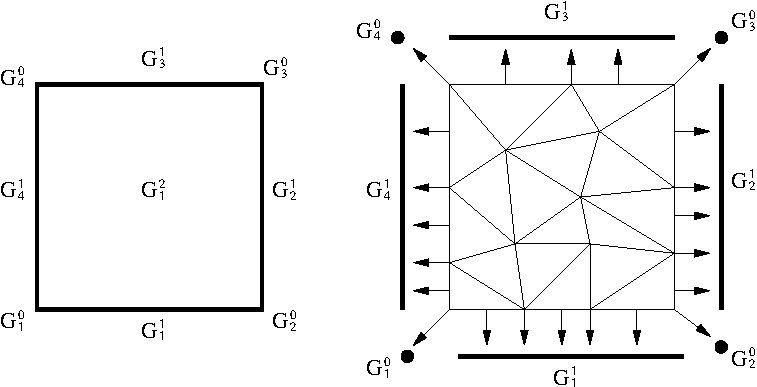
\includegraphics[width=4in]{../fig/gclas}
\caption[Example of simple model and mesh showing their association via geometric classification]
{Example of simple model(left) and mesh(right) showing
their association via geometric classification~\cite{simmetrixweb}} 
\label{gclas}  % the \label command comes AFTER the caption
\end{figure}

The unique association of a mesh entity of dimension \di, \Mdii, to the
 geometric model entity of dimension \djj, $G^{d_j}_j$, $d_i \le d_j$, on which
 it lies is termed geometric classification, and is denoted \Mdiib\clas\blk
 $G^{d_j}_j$, where the classification symbol, \clas,
indicates that the left hand entity, or a set of entities, is classified on the right hand entity. In Figure \ref{gclas}, a mesh of simple square model with entities labeled
is shown with arrows indicating the classification of the mesh entities onto the model
entities. All of the interior mesh faces, mesh edges, and mesh vertices are classified
on the model face $G^2_1$.

%%%%%%%%%%%%%%%%%%%%%%%%%%%%%%%
\subsubsection{Adjacencies}
%%%%%%%%%%%%%%%%%%%%%%%%%%%%%%%
\begin{figure}
\centering
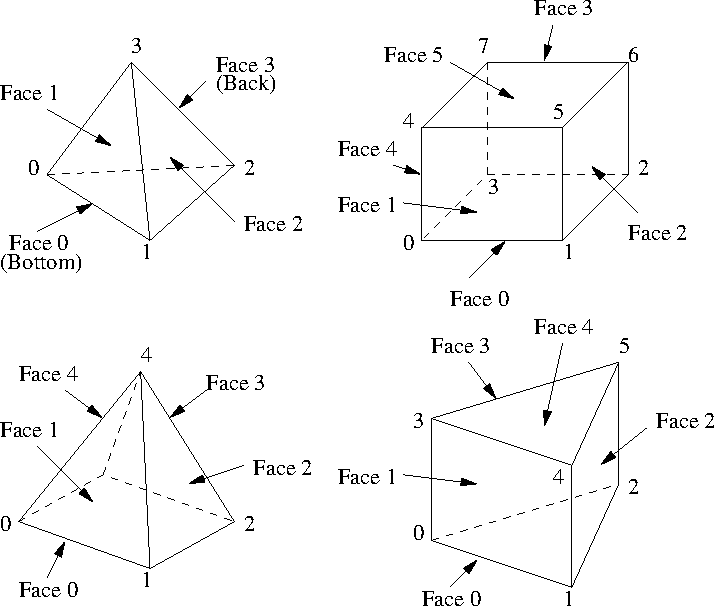
\includegraphics[width=4in]{../fig/rorder-vf}
\caption[Vertex and face order on a region]
{Vertex and face order on a region~\cite{simmetrixweb}}
\label{rorder1}  
\end{figure}

\begin{figure}
\centering
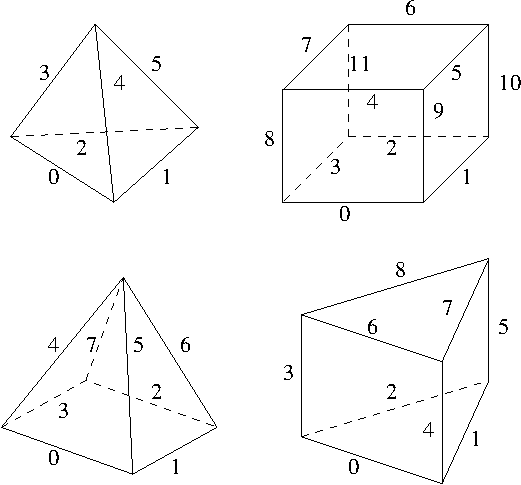
\includegraphics[width=3in]{../fig/rorder-e}
\caption[Edge order on a region]
{Edge order on a region~\cite{simmetrixweb}}
\label{rorder2}  
\end{figure}

\begin{figure}
\centering
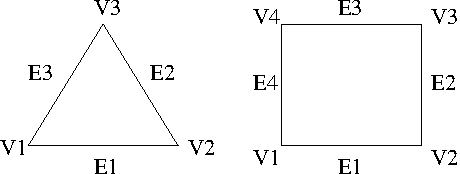
\includegraphics[width=3in]{../fig/forder}
\caption[Edge order on a face]
{Edge order on a face~\cite{simmetrixweb}}
\label{forder}
\end{figure}

\begin{figure}
\centering
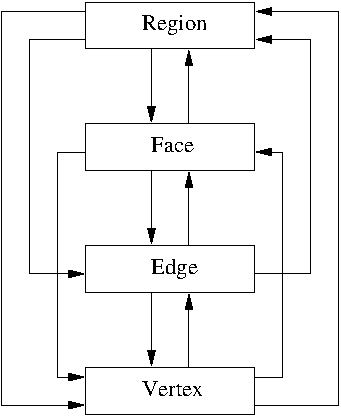
\includegraphics[width=1.5in]{../fig/12adj}
\caption[12 adjacencies possible in the mesh representation]
{12 adjacencies possible in the mesh representation~\cite{garimella02}}
\label{12adj}  % the \label command comes AFTER the caption
\end{figure}

Adjacencies describe how mesh entities connect to each other. For
an entity of dimension $d$, first-order adjacency returns all of
the mesh entities of dimension $q$, which are on the closure of the
entity for a downward adjacency ($d>q$), or for which the entity is
part of the closure for an upward adjacency ($d<q$). For denoting specific downward
first-order adjacent entity,
$M^d_i\{M^q\}_j$, the ordering conventions can be used to enforce the
order. Figure \ref{rorder1}, \ref{rorder2}, and \ref{forder} illustrate a
common canonical order of bounding entities. Figure~\ref{12adj} is an
adjacency graph that depicts 12 first-order adjacencies possible in 
the mesh data structure where a solid box and a solid arrow
denote, respectively, explicitly stored level of entities and explicitly stored adjacencies from
outgoing level to incoming level. In the adjacency graph, a solid box denotes that entities of the level are explicitly stored, and a solid arrow denotes that adjacencies from an outgoing level to an incoming level are maintained for the level of entities.

For an entity of dimension $d$, second-order adjacencies describe
all the mesh entities of dimension $q$ that share any adjacent
entities of dimension $b$, where $d \neq b$ and $b \neq q$. Second-order
adjacencies can be derived from first-order adjacencies. 

Examples of adjacency requests include: for a given face, the regions
on either side of the face (first-order upward); the vertices bounding
the face (first-order downward); and the faces that share any vertex
with a given face (second-order). 

%%%%%%%%%%%%%%%%%%%%%%%%%%%%%%%%%%%%%%%%%%%%%%%%%%%%%%%%%%%%%%
\subsubsection{Mesh Representation}\label{ch:meshrep}
%%%%%%%%%%%%%%%%%%%%%%%%%%%%%%%%%%%%%%%%%%%%%%%%%%%%%%%%%%%%%%
The mesh representation can be categorized with two criteria (i) full vs. reduced and (ii) complete vs. incomplete, resulting in 4 different groups~\cite{seolthesis}. 

If a mesh representation stores all $0$ to $d$ level entities explicitly, it is a $full$ representation, otherwise, it is a $reduced$ representation. \emph{Completeness of adjacency} indicates the ability of a mesh representation
to provide any type of adjacencies requested without involving an
operation dependent on the mesh size such as the global mesh search or mesh traversal.
Regardless of full or reduced, if all adjacency information is obtainable in
O(1) time (the first circle), the representation is \emph{complete}, otherwise it is \emph{incomplete}. 

The \emph{general} topology-based mesh data structures must satisfy completeness of adjacencies to support adaptive
analysis efficiently. It doesn't necessarily mean that all $d$ level entities and adjacencies need be explicitly stored in the representation so there are many representation options in the design of general topology-based mesh data structure. 
\begin{figure}
\centering
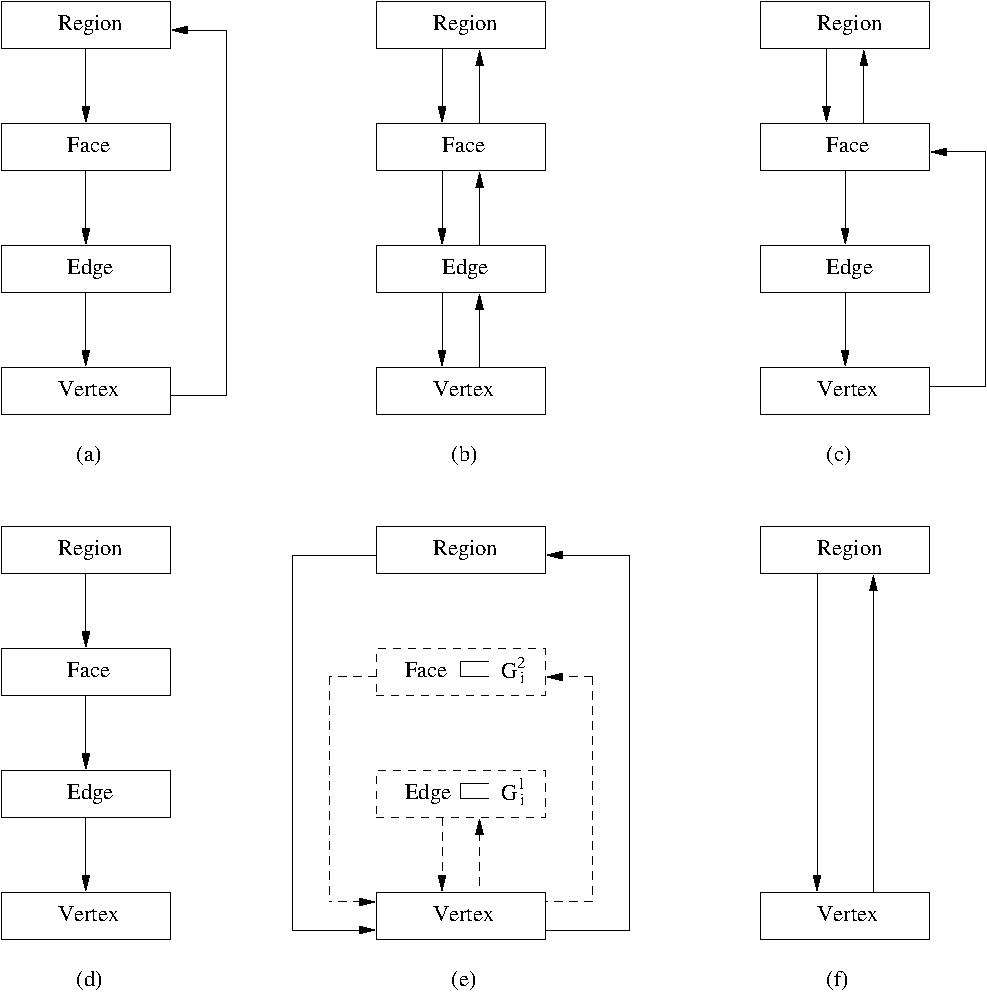
\includegraphics[width=4.2in]{./fig/6complete}
\caption{Example of 3D mesh representations}
\label{fig:6completeMR}  
\end{figure}

In the mesh representation graph, a dotted box denotes that among entities of the level, only equally
classified ones are explicitly stored, and a dotted arrow denotes that adjacencies
from an outgoing level to an incoming level are maintained only for the stored
entities.

In Figure \ref{fig:6completeMR} illustrates 6 mesh representations in 3D. Note that in the adjacency graph, a dotted box denotes that among entities of the level, only equally
classified ones are explicitly stored, and a dotted arrow denotes that adjacencies
from an outgoing level to an incoming level are maintained only for the stored
entities. (a) to (c) are full and complete due to all $0$ to $d$ levels of entities exist and the 12
adjacencies are obtainable in O(1) time either by direct access or local
traversal, (d) is full and incomplete
since it requires mesh level global search or traversal to get proper
adjacencies, (e) is reduced and complete, and (f) is reduced and incomplete. Representation (b) is \emph{the one-level adjacency representation} as it maintains adjacencies between entities one dimension apart. Representation (e) is \emph{the complete minimum sufficient representation} that
stores the minimum sufficient representation plus upward adjacencies from
vertices to their bounding entities of level $>$ 0. Representation
(f) is the classic mesh connectivity structure 
that describes the mesh only in terms of elements and nodes, and also has been used
for several finite element applications~\cite{beall97}.

For more discussions on mesh representations, see Reference ~\cite{seolthesis}.

%%%%%%%%%%%%%%%%%%%%%%%%%%%%%%%
\subsubsection{Entity set}
%%%%%%%%%%%%%%%%%%%%%%%%%%%%%%%

An entity set provides a mechanism for creating arbitrary groupings of entities for various purposes such as representing boundary layer, boundary condition and materials. Each entity set can be either of a set with unique entity or a list with insertion order preserved. The following are the functionalities of entity set to effectively support the application needs~\cite{itapsweb, Ollivier-etal06}.
 
\begin{itemize}
\item populating by addition or removal of entities from the set
\item traversal through an iterator with various conditions such as topology, and type of the entity
\item set boolean operations of subtraction, intersection, and union
\item relationships among entity sets: subset, parent/child
\end{itemize}

In parallel computing environment, the mesh is distributed over multiple parts across the processes. Therefore, there are two kinds of set available in distributed mesh.
\begin{itemize}
\item mesh set: entity set created in a mesh. entities in the set can be in different part.
  \begin{itemize}
    \item $L-SET$: a list type entity set created in mesh. Insertion order is preserved and an entity can be inserted multiple times.
    \item $S-SET$: a set type entity set created in mesh. Insertion order is not preserved and an entity can be inserted at most once.
\end{itemize}
\item  part set or $P-SET$: a set type entity set created in part. Insertion order is preserved and only entities ithout higher order adjacency can be inserted. 
\end{itemize}

Please be noted that entity set is not supported in the current PUMI release.

%%%%%%%%%%%%%%%%%%%%%%%%%%%%%%%
\subsubsection{Iterator}
%%%%%%%%%%%%%%%%%%%%%%%%%%%%%%%

Iterators are a generalization of pointers which are objects that point to other objects. Iterators are often used to iterate over a range of objects: if an iterator points to one element in a range, then it is possible to increment it so that it points to the next element~\cite{sgiweb}. 

Various kinds of iterators are desirable for efficient mesh entity traversal with various conditions such as entity dimension, entity topology, geometric classification. Furthermore, the iterator validity shall be guaranteed with mesh modification through entity creation/deletion.

%%%%%%%%%%%%%%%%%%%%%%%%%%%%%%%
\subsubsection{Tag}\label{tag}
%%%%%%%%%%%%%%%%%%%%%%%%%%%%%%%

A tag is a container of arbitrary data attachable to meshes, entities, and entity sets. Different values of a particular tag can be associated with mesh, entity, or entity set~\cite{itapsweb, Ollivier-etal06}. 

For efficient manipulation of tags and their association with meshes, entities and entity sets, tags consist of the following data.
\begin{itemize}
\item{tag name}: character string for identifying tag
\item{tag data}: data stored in the tag
\item{tag type}: data type for tag data \\
For better performance and management, five specialized tag types, integer, double, mesh entity, entity set and byte type data are supported through interface. If the tag data consists of multiple units (e.g. array of integer data), the size of tag data in byte and  the number of units are needed for efficient tag manipulation.
\item{tag size}: the number of units of \emph{tag type} in tag data
\item{tag byte}: the size of tag data in bytes
\end{itemize}

%%%%%%%%%%%%%%%%%%%%%%%%%%%%%%%
\subsection{S/W Structure}
%%%%%%%%%%%%%%%%%%%%%%%%%%%%%%%

\begin{figure}[!t]
\centering
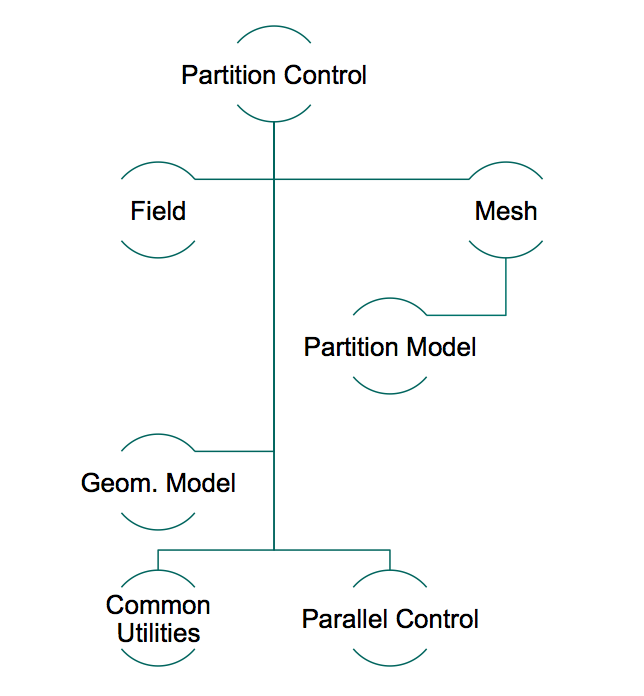
\includegraphics[width=3in]{fig/pumi.jpg} 
\caption{Software structure of PUMI}
\label{fig:pumi}
\end{figure}

In development, geometry-based analysis s/w is modularized based on the features and goals as component. Figure~\ref{fig:pumi} illustrates the software structure of PUMI consisting of the following seven components. % add some additional discussion of the interactions implied in the figure
\begin{itemize}
\item The \emph{common utility} component provides common utilities and services used in multiple other components such as iterator, set, and tag.
\item The \emph{parallel control} component provides parallel-specific utilities and services such as communications and architecture-aware operations.
\item The \emph{geometric model} component provides a uniform interface for querying geometric model representations. It uses common utility and parallel control component. 
\item The \emph{partition model} component is constructed based on the mesh distribution and provides mesh partitioning representation in topology to the mesh component for the support for efficient update/manipulation of mesh with respect to partitioning. 
\item The \emph{mesh} component provides the storage and management of distributed unstructured meshes. It uses all components except for  the field component.
\item The \emph{field} component provides the services for storage and management of solution information on the mesh. It uses common utility, parallel control and mesh components.
\item The \emph{partition control} component provides the services for improving mesh partitioning via graph partitioner or existing mesh information such as adajacencies.
\end{itemize}


PUMI consists of multiple libraries which are modularized based on supported features. 

\begin{itemize}
\item \texttt{pumi}: a library with API hearder file and PUMI error codes. PUMI error codes are defined in the file \texttt{pumi\_errorcode.h} and the API's are defined in the file \texttt{pumi.h}.
\item \texttt{pcu}: a library with parallel control and comminication. The header file is obtained in \texttt{PCU.h}.
\item \texttt{gmi}: a library with SCOREC-formatted geometric model implementation. 
\item \texttt{mds}: a library with SCOREC-formatted mesh implementation. 
\item \texttt{apf}: a library with field, common mesh interface, common geometric model interface, interations between geometric model and mesh implmentation, etc. The header file is obtained in \texttt{apf.h}.
\item \texttt{parma}: a library with adjacency-based mesh partitioning functions. The header file is obtained in \texttt{parma.h}.
\item \texttt{zoltan}: a library to support interaction with Zoltan~\cite{ZoltanIsorropiaOverview2012, ZoltanOverviewArticle2002} graph partitioning S/W.
\end{itemize}

